\chapter{The Mathematics of Nature}
\label{chap:X_mathematics_of_nature}

% =====================================================
% 10.1 Introduction: Visible Nature, Hidden Order
% =====================================================

\subsection{Introduction: Visible Nature, Hidden Order}

When people think of mathematics, they often think of numbers, formulas, and abstract concepts.
Nature, by contrast, initially appears different:
diverse, irregular, alive, and often difficult to calculate.
Trees do not grow like ideal lines,
clouds have no exact contours,
rivers follow no ruler,
and even flowers or crystals may show order,
but never in the perfect purity of a textbook image.
For this very reason, the visible world at first glance
seems almost the opposite of mathematical rigor.

But this impression is misleading.
Behind the diversity of nature there are often structures
that can be described mathematically.
This structure does not always appear in perfect regularity,
but often in recurring patterns,
in functional compromises,
in symmetries,
growth processes,
or energetically favorable forms.
The mathematics of nature therefore lies not only in ideal figures,
but precisely in the lawful relationships
that bring real forms into being.

Thus honeycombs do not arise as decorative patterns,
but as efficient structures with low material use.
Branching in trees,
blood vessels, or river systems
does not merely follow random growth,
but functional requirements of supply,
stability, and transport.
Snowflakes and crystals show symmetries
that arise from the properties of their microscopic building blocks.
Spirals in plants or patterns on animal coats arise from local rules
that, in combination, produce visible order.

In all these cases, mathematics does not simply describe something
that one would already have fully understood anyway.
Rather, it makes precisely visible
which structure is at work behind the forms.
It shows
why certain shapes occur preferentially,
which conditions guide their growth,
and why, among many possibilities, only a few stable
or efficient patterns prevail.
Here mathematics is not merely language,
but an instrument of knowledge.

At the same time, nature must not be confused with an idealized textbook.
Real systems are imperfect,
disturbed,
historically grown,
and shaped by many influences.
Precisely for this reason, it is important
to distinguish between mathematical model and concrete reality.
Mathematics does not capture every detail,
but it uncovers orders
hidden within what appears accidental.

This chapter therefore deliberately returns to the visible world.
After the historical,
philosophical,
and modern perspectives of the preceding chapters,
concrete examples will now show
how mathematical structure emerges in nature.
The aim is not
to reduce reality to formulas,
but to make visible
that natural forms,
growth processes,
and orders often follow mathematically describable relationships.
Here again, the guiding idea of this book is confirmed:
the world is not mathematically decorated,
but mathematically structured.

\begin{DidacticBox}[Nature and Mathematical Structure]
	\phantomsection\label{box:nature-structure}
	Mathematics appears in nature not only in perfect forms,
	but also in growth processes,
	symmetries,
	optimizations,
	and recurring patterns.
	Precisely where the visible world appears irregular,
	mathematical description can make the hidden order visible.
\end{DidacticBox}

% =====================================================
% 10.2 Honeycombs and the Principle of the Optimal Form
% =====================================================

\subsection{Honeycombs and the Principle of the Optimal Form}
\index{honeycomb}
\index{geometry}
\index{lightweight construction}
\index{optimization}
\index{honeycomb structure}

Honeycombs are approximately hexagonal.
This is not merely a decorative form,
but an expression of geometric efficiency.
Regular hexagons can fill a plane without gaps
and, for a given cell size, require relatively little wall length.
This creates a structure
that provides a large number of stable cells
with little material use.

Here a fundamental mathematical principle becomes visible:
under given conditions, not just any form prevails,
but one
that fulfills certain requirements especially well.
In the case of the honeycomb, the issue is a compromise between stability,
space utilization,
and material savings.
The hexagonal structure is therefore not a random whim of nature,
but a form
that proves itself functionally.

The same principle is also found in engineering.
In lightweight construction,
especially in aerospace engineering,
so-called honeycomb cores are used as the core of sandwich components.
Two thin,
strong face sheets are kept apart by a lightweight core.
The honeycomb core stabilizes against buckling
and absorbs shear forces,
while the face sheets carry tensile and compressive forces under bending.
This produces very high bending stiffness at low weight.

This makes visible
that the same geometric idea is effective in nature and technology.
What appears in the beehive as a natural structure
is deliberately used in engineering as a design principle.
Here mathematics appears not only as the description of an existing form,
but as insight into an ordering principle
that can be applied in practice.

\begin{NoteBox}[The Bee Does Not Calculate -- But the Structure Arises]
	\phantomsection\label{box:bee-structure}
	\small
	The honeycomb shows
	that mathematical structure does not begin only in human thought.
	When material,
	forces,
	and boundary conditions interact,
	stable geometric forms often arise in nature.
	Mathematics is then not merely invention,
	but the precise instrument
	with which we recognize,
	describe,
	and technically use such structures --
	from the beehive to sandwich structures in lightweight construction.
\end{NoteBox}

\begin{figure}[htbp]
	\centering
	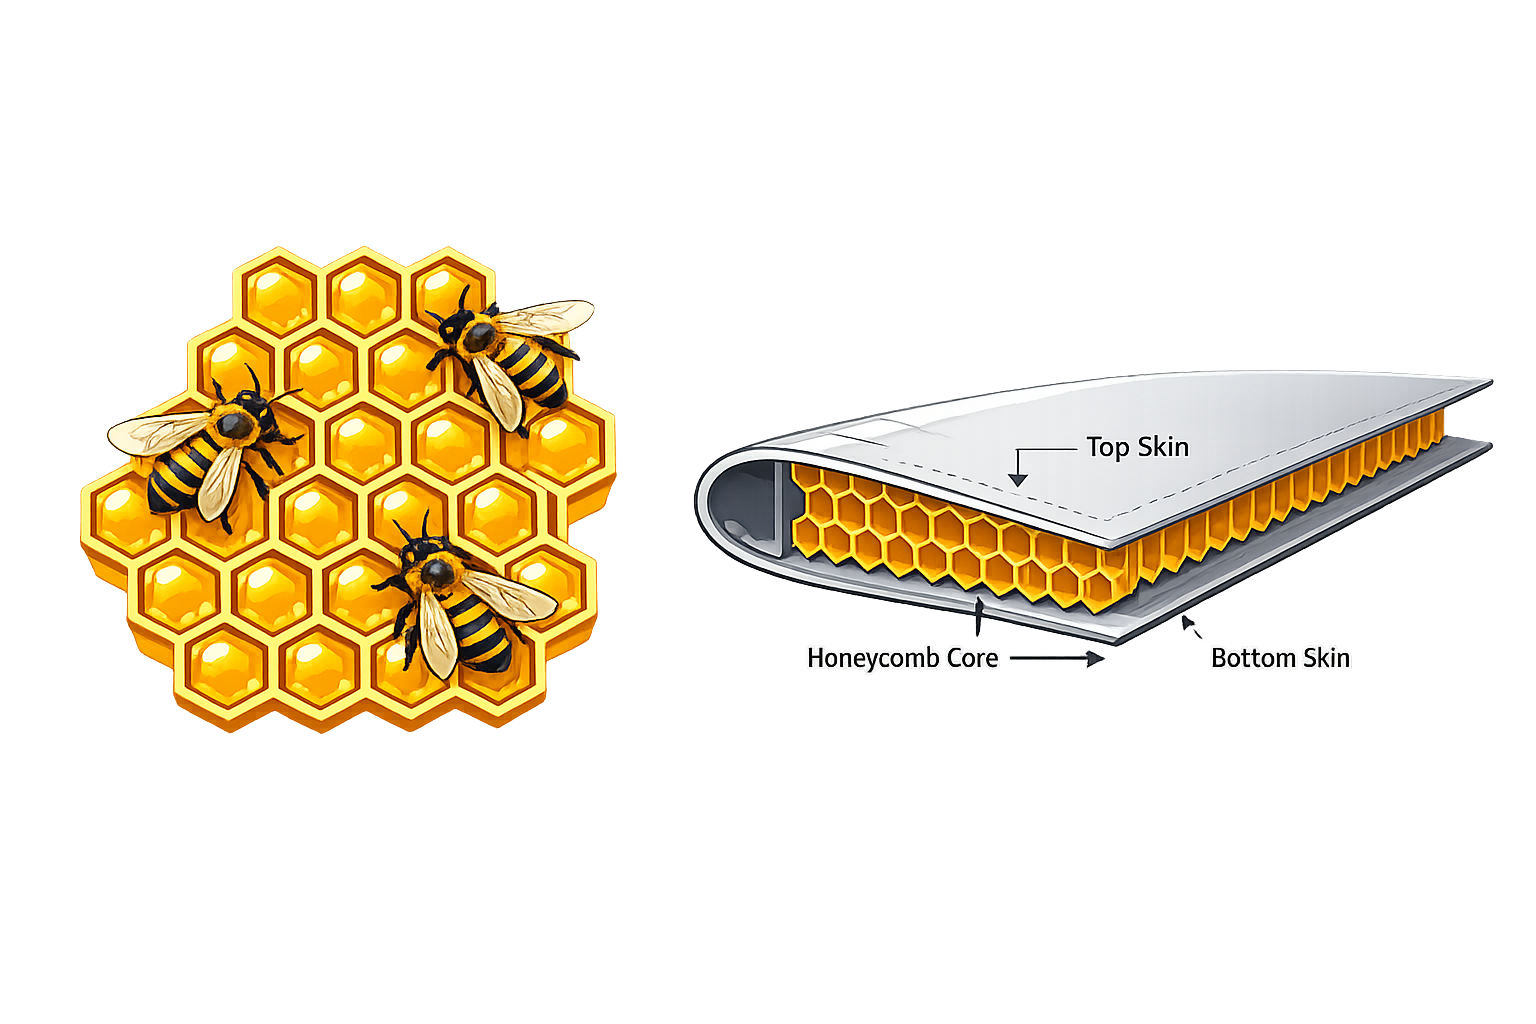
\includegraphics[width=0.85\linewidth]{bilder/Bienen.png}
	\caption{Honeycombs and technical lightweight construction: the same structural idea in nature and engineering.}
	\label{fig:waben_leichtbau}
\end{figure}

\newpage
\noindent

% =====================================================
% 10.3 Branching Networks in Nature and Engineering
% =====================================================

\subsection{Branching Networks in Nature and Engineering}
\index{branching}
\index{network}
\index{tree}
\index{biology}
\index{optimization}
\index{string theory}
\index{minimal surfaces}

Branching networks are among the most impressive forms of natural order.
They are found in trees,
root systems,
blood vessels,
bronchi,
river systems,
or nerve cells.
At first glance, such structures often appear irregular.
On closer inspection, however, they show a recurring principle:
a main branch divides into smaller units,
which in turn branch further.
This creates a network
that enables supply,
transport,
or distribution with the least possible effort.

Botany provides an intuitive example.
With its crown, a tree maximizes the absorption of light,
but at the same time must transport water and nutrients through a branching conduit system
to great heights.
The resulting form is therefore not accidental,
but the result of a compromise between growth,
supply,
material use,
and mechanical stability.
Exactly such conflicts of objectives can be described mathematically as optimization problems.

\begin{DidacticBox}[Not Chance, But Functional Structure]
	\phantomsection	\label{box:branching-network}
	Branching forms in nature do not arise
	because an organism ``calculates.''
	They arise
	because transport,
	stability,
	material use,
	and growth must be fulfilled at the same time.
	Mathematics makes these conflicts of objectives visible
	and describes
	why certain network forms are especially favorable under given conditions.
\end{DidacticBox}

Such networks are not only biologically interesting,
but also technically significant.
The same questions arise in supply networks,
traffic routes,
pipe systems,
or distribution structures:
How can something be distributed efficiently
without wasting unnecessary material,
energy,
or space?
Here it becomes clear
that mathematical concepts such as optimization,
network structure,
and minimality are not bound to a particular material,
but to the form of the relationships themselves.

In the twenty-first century, this method transfer has become especially fruitful.
Mathematical tools
that were originally developed in highly abstract fields
are now applied to real network problems.
For example, methods from the theory of minimal surfaces,
geometric optimization,
or even from the environment of string theory
can be used
to investigate the geometry of branching tube networks.
This does not mean
that a tree or a blood vessel ``consists of strings.''
What matters instead
is that the same mathematical structural problems reappear
in very different contexts.

Precisely here the reach of mathematical thinking becomes visible.
A branching network is not only a biological or technical object,
but an example of how nature repeatedly solves problems of supply,
stability,
and efficiency.
Here mathematics does not merely describe a visible form,
but the hidden order
that brings this form into being.
A more detailed mathematical treatment of such a branching network
follows in Appendix~\ref{app:netzwerke-minimalflaeche}.

\begin{figure}[htbp]
	\centering
	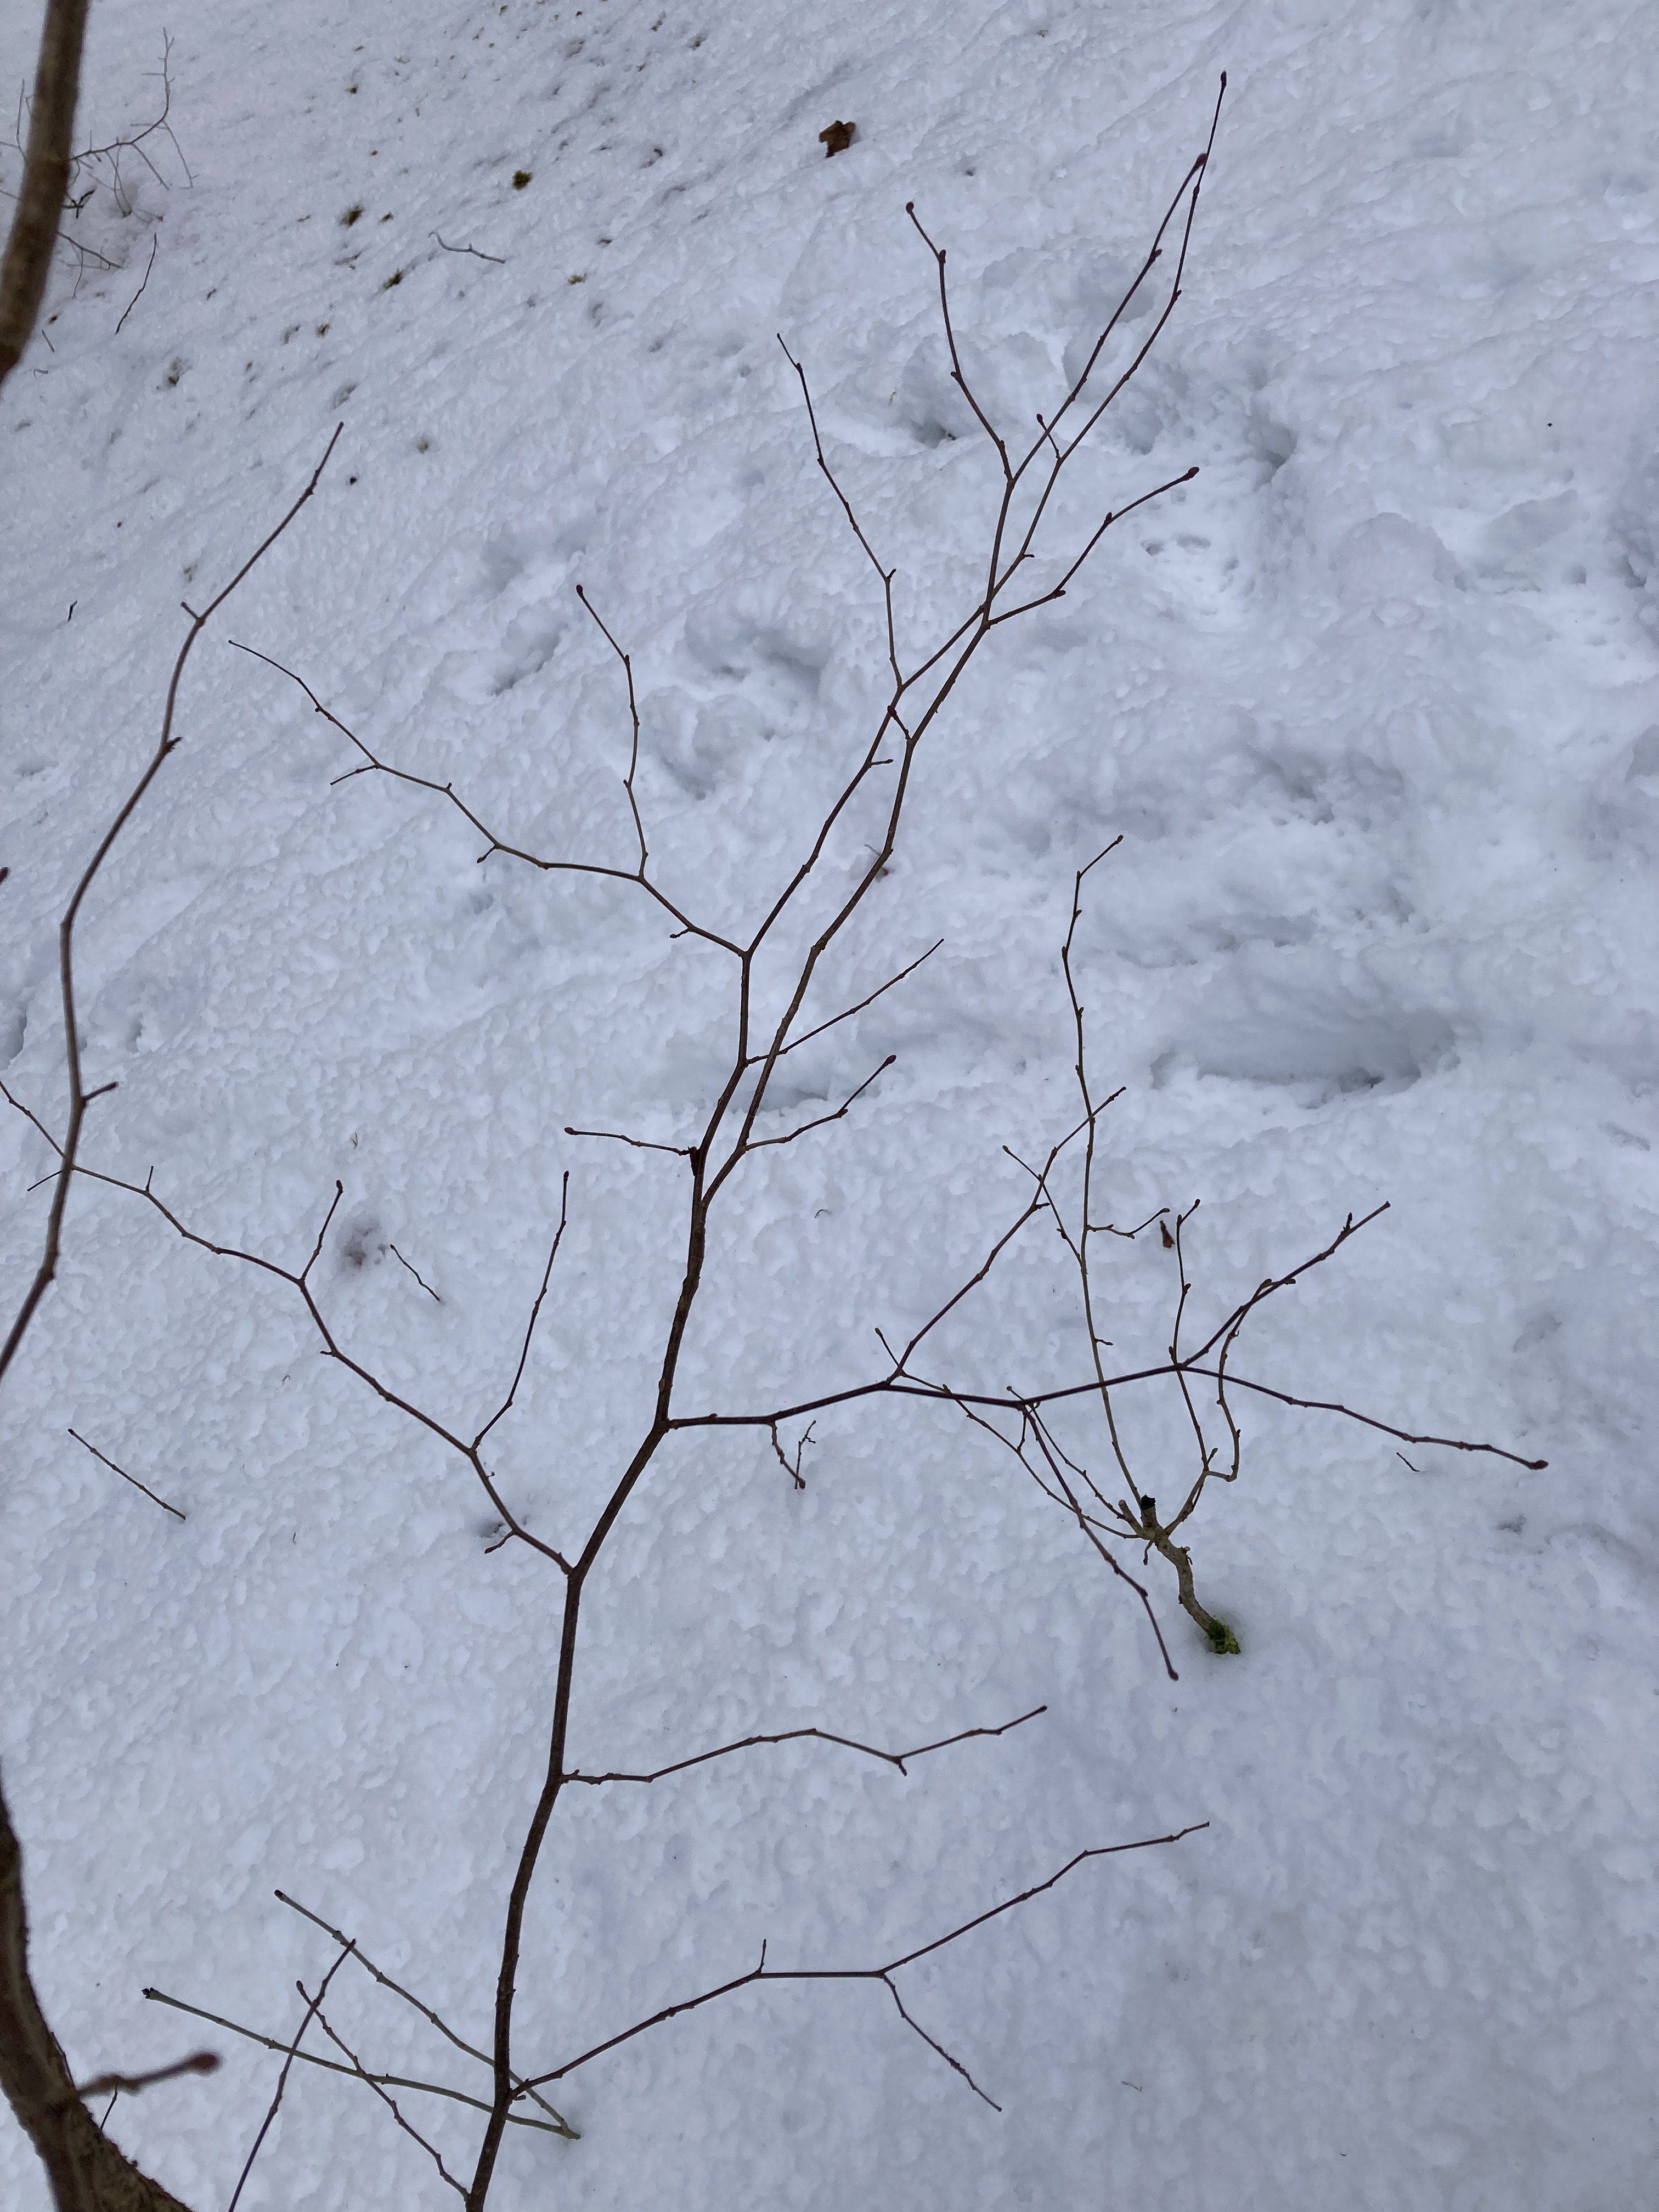
\includegraphics[width=0.62\linewidth]{bilder/Baum.png}
	\caption{Branching structure of a young tree. What becomes visible here is not only a botanical form, but a natural network whose shape can be understood as a compromise between growth, supply, and stability.}
	\label{fig:baum-verzweigung}
\end{figure}

\newpage
\noindent

% =====================================================
% 10.4 Spirals and Leaf Arrangements in Plants
% =====================================================

\subsection{Spirals and Leaf Arrangements in Plants}
\index{spiral}
\index{leaf arrangement}
\index{plant}
\index{Fibonacci sequence}
\index{phyllotaxis}
\index{growth}
\index{optimization}

In the plant world as well, mathematics appears not only in ideal figures,
but in real growth processes.
This is especially striking in spirals and leaf arrangements.
Leaves are often not positioned randomly on a stem,
but in an arrangement
that prevents them from shading one another too strongly.
Similar patterns are found in sunflowers,
pine cones,
pineapples,
or cacti,
where seeds,
scales,
or leaves are arranged in clearly recognizable spiral structures.

In botany, such arrangements are grouped under the term \emph{phyllotaxis}.
This refers to the regular positioning of leaves,
buds,
or other plant parts along a growth axis.
This becomes mathematically interesting
because surprisingly ordered overall patterns arise
from simple local growth rules.
New leaves or seeds appear at positions
that avoid already existing structures.
As a result, the available space is used as evenly as possible.

The connection to the Fibonacci sequence is especially well known in this context.

\begin{NoteBox}[Fibonacci and Plants]
	\phantomsection\label{box:fibonacci-plants}
	The Fibonacci numbers appear in plants not as a conscious calculation procedure,
	but as a consequence of certain growth and packing rules.
	A brief mathematical explanation can be found in
	Appendix~\ref{app:fibonacci-goldener-schnitt}.
\end{NoteBox}

\newpage
\noindent

As can be seen in Figure~\ref{fig:sunflower-fibonacci},
sunflowers form ordered spiral structures
that are often connected with Fibonacci numbers.

\begin{figure}[htbp]
	\centering
	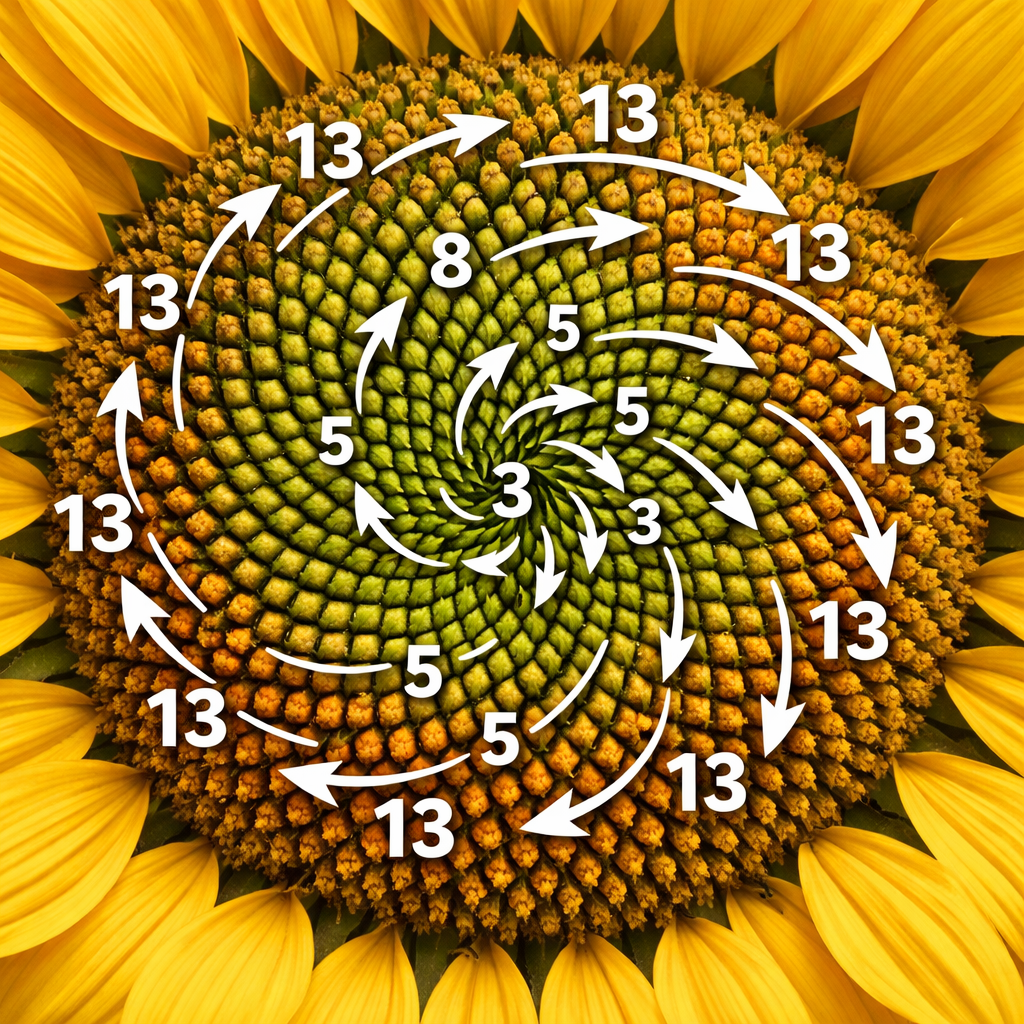
\includegraphics[width=0.82\linewidth]{bilder/sunflower.png}
	\caption{Sunflower with visible spiral structures. Such arrangements are connected with growth rules and efficient space distribution; spiral numbers often occur that are linked to the Fibonacci sequence.}
	\label{fig:sunflower-fibonacci}
\end{figure}

When one counts the visible spirals in opposite directions in many plants,
numbers such as 3 and 5,
5 and 8,
or 8 and 13 often occur.
This observation is fascinating,
but it should be understood soberly.
The plant does not ``know'' the Fibonacci sequence.
Rather, certain growth rules and packing conditions lead
to spiral numbers
that often agree with this sequence.

\begin{DidacticBox}[Do Not Understand Fibonacci Mystically]
	\phantomsection\label{box:fibonacci-mystical}
	Fibonacci numbers in plants are not a secret law of nature
	and not a magical formula.
	They appear where local growth rules,
	space distribution,
	and mutual displacement interact.
	Mathematics describes this pattern,
	but it is not consciously ``applied'' by the plant.
\end{DidacticBox}

This is precisely where the mathematical significance of such forms lies.
The visible spirals are not merely beautiful to look at,
but expressions of an ordering principle.
The point is efficient use of space,
uniform distribution,
and growth rules
that together generate a stable structure.
Once again it becomes visible:
mathematics does not lie only in later description,
but in the structure of the process itself.

At the same time, real plants are not perfect textbook objects.
Light,
wind,
injuries,
irregular growth,
and environmental conditions mean
that no plant looks perfectly ideal.
This is exactly what makes the mathematical approach interesting:
it does not search for absolute perfection,
but for the structure
that persists under changing conditions.

Spirals and leaf arrangements in plants are therefore an especially intuitive example
of how ordered forms arise from simple local rules.
Here mathematics appears not as a rigid scheme,
but as the description of a dynamic growth process.
Again it becomes visible
that natural forms are not mathematically decorated,
but mathematically structured.

% =====================================================
% 10.5 Minimal Surfaces and Energetically Favorable Forms
% =====================================================

\subsection{Minimal Surfaces and Energetically Favorable Forms}
\index{minimal surface}
\index{soap film}
\index{energy}
\index{surface tension}
\index{optimization}
\index{geometry}

Not only fixed structures such as honeycombs or branching networks show mathematical order.
Fluid systems also produce forms
that can be understood only
when one asks about the most favorable state.
Soap films provide an especially intuitive example.
If one dips a wire frame into soapy water
and pulls it out again,
a thin film forms
that fills the boundary.
This form is not accidental.
It arises
because surface tension tends to keep the area of the film as small as possible.

Here a central mathematical principle becomes visible:
under given boundary conditions,
the form that often prevails
is the one that minimizes a certain quantity.
In the case of the soap film, this quantity is surface area.
Such surfaces are called \emph{minimal surfaces}.
They are not arbitrary geometric shapes,
but real forms
that arise from an energetically favorable state.

\begin{DidacticBox}[Why Soap Films Are Mathematically Interesting]
	\phantomsection\label{box:soapfilm}
	A soap film does not consciously ``search'' for the best form.
	It assumes that form
	because surface tension energetically favors states with smaller area.
	Mathematics describes this process not from the outside as a mere picture,
	but as an optimization problem with clear boundary conditions.
\end{DidacticBox}

This makes soap films an ideal example
of the connection between nature and mathematics.
A physical process directly realizes a geometric extremal property.
This makes visible
that optimization is not a thinking scheme invented afterward,
but is effective in nature itself.
Energy,
form,
and geometry are closely connected here.

Such minimal principles play a role far beyond the simple example of a soap film.
Drops,
membranes,
and many interfaces in nature and engineering
also assume forms
determined by energetic favorability.
The visible shape then results not from chance,
but from an interplay of forces,
boundary conditions,
and stability.
Mathematics makes these relationships precisely describable.

At the same time, this example shows an important limit of mere intuition.
At first glance, a soap film appears simple and self-evident.
Yet its exact form can be mathematically highly demanding,
especially for complicated boundary curves.
Here again it becomes clear:
nature often realizes a structure directly,
while its exact mathematical description requires deep insights
and sophisticated methods.

Minimal surfaces and energetically favorable forms
therefore make a basic feature of reality visible.
The world is not only full of forms;
many of these forms arise
because under given conditions certain states are favored.
Mathematics therefore does not merely describe what is visible,
but the hidden principles
by which it forms.
Here again it becomes clear
that nature is not mathematically decorated,
but mathematically structured.

\begin{figure}[htbp]
	\centering
	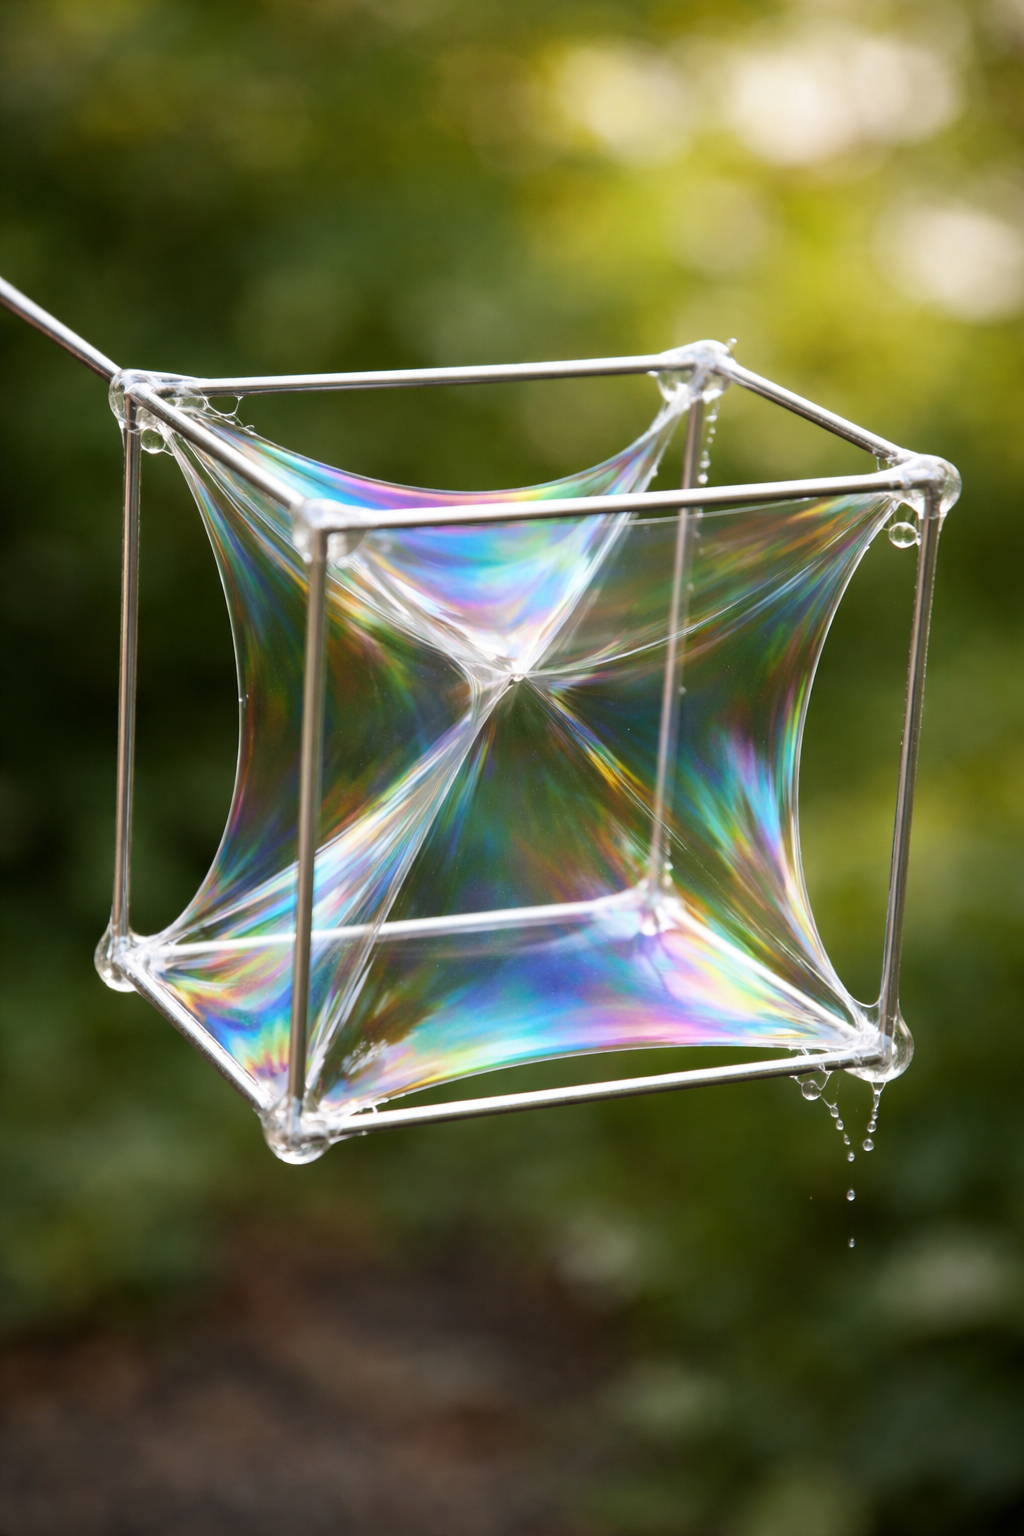
\includegraphics[width=0.62\linewidth]{bilder/seifenfilm.png}
	\caption{Soap film in a cube-shaped wire frame. The resulting form is not accidental, but follows from the tendency of the system to assume the smallest possible surface area under given boundary conditions.}
	\label{fig:seifenfilm-drahtrahmen}
\end{figure}

% =====================================================
% 10.6 Symmetry in Crystals and Snowflakes
% =====================================================
\newpage
\noindent
\subsection{Symmetry in Crystals and Snowflakes}
\index{symmetry}
\index{crystal}
\index{snowflake}
\index{geometry}
\index{natural form}
\index{structure}

Symmetry is one of the most striking signs of mathematical order in nature.
Wherever parts of an object recur in a certain way,
can be reflected,
or rotated
without the basic form being lost,
a structure becomes visible
that can be described mathematically with precision.
This order appears especially clearly
in crystals and snowflakes.

Crystals do not arise in arbitrary forms.
Their external shape is connected
with the regular arrangement of their building blocks inside.
Atoms or molecules arrange themselves in lattice structures,
and this internal symmetry also shapes the external form of the crystal.
Thus an important connection becomes visible:
visible order on the surface is often an expression of a deeper,
invisible order within.

Snowflakes are an especially intuitive example.
They appear in countless variations,
and yet almost always possess a sixfold basic symmetry.
This form goes back to the structure of water
and the way water molecules arrange themselves during freezing.
The individual arms of a snowflake grow under similar conditions,
so that a common basic order is preserved.
At the same time, small differences in temperature,
humidity,
and motion mean
that no snowflake is perfectly identical to another.

\begin{DidacticBox}[Symmetry and Variation]
	\phantomsection\label{box:symmetry-variation}
	The mathematical order of nature does not mean
	that everything must be perfectly identical.
	Snowflakes in particular show
	that a clear basic symmetry can coexist with individual variety.
	Structure and variation do not exclude one another.
\end{DidacticBox}

Precisely therein lies the mathematical significance of such forms.
Symmetry does not merely mean beauty or regularity in an aesthetic sense.
It indicates
that under certain transformations
something essential remains unchanged.
In crystals and snowflakes, this invariance is not imposed from outside,
but grows out of the physical conditions of the substances themselves.

For understanding nature, this is highly significant.
Symmetries make it possible
to trace complicated forms back to a few basic structural principles.
They make visible
that behind the diversity of appearances
there are often simple orders.
Mathematics grasps these orders not as mere decoration,
but as expressions of inner lawfulness.

Crystals and snowflakes are therefore far more
than beautiful natural forms.
They show
that the world is shaped by mathematically describable structures
not only on large scales,
but also on small ones.
Precisely in the connection between rule and deviation,
between symmetry and individual expression,
it becomes visible
how deeply mathematical order reaches into nature.

\begin{figure}[htbp]
	\centering
	
\includegraphics[width=0.62\linewidth]{bilder/schneeflocke.png}
	\caption{Macro photograph of a snowflake with clearly visible sixfold symmetry. Despite individual differences, its basic form follows a clear geometric order that arises from the structure of water and the conditions of crystal growth.}
	\label{fig:schneeflocke-symmetrie}
\end{figure}

\newpage
\noindent

% =====================================================
% 10.7 Pattern Formation and Self-Organization
% =====================================================

\subsection{Pattern Formation and Self-Organization}
\index{pattern formation}
\index{self-organization}
\index{order}
\index{nature}
\index{reaction-diffusion system}
\index{dynamics}

Not all mathematical structures in nature are imposed from outside.
Many arise from the interplay of simple local processes
that lead to ordered overall patterns without a central plan.
This is precisely what is called \emph{self-organization}.
It means the emergence of order from internal dynamics:
from many small interactions, a larger structure forms
without that structure having to be completely specified from outside.

Such processes are found in very different areas of nature.
Stripes and spots on animal coats,
wave patterns in sand dunes,
ripple structures on water surfaces,
or spatial patterns in chemical reactions show
that order is not always the result of a fixed construction plan.
Often it is enough
for simple rules to act locally
and influence one another.
From this interaction, forms arise
that appear clearly ordered on a larger scale.

A classic example is provided by so-called reaction-diffusion systems.
In these systems, substances spread through space,
react with one another,
and mutually influence one another.
Even a few equations can thereby produce stable spots,
stripes,
or wave-like patterns.
What is especially remarkable mathematically
is that complex visible structures can arise
from relatively simple rules.

\begin{DidacticBox}[Order Without a Central Construction Plan]
	\phantomsection\label{box:selforganization}
	Self-organization does not mean chaos,
	but ordered structure from local interaction.
	A pattern therefore does not have to be designed from outside.
	It can arise by itself from simple rules
	if the dynamics of the system allow it.
\end{DidacticBox}

This is where the deep mathematical meaning of such phenomena lies.
Mathematics here describes not only a finished form,
but the process of its emergence.
What matters is not only
what a pattern looks like,
but which equations,
feedbacks,
and stability conditions cause it
to form and persist.
The order therefore lies not only in the result,
but in the law of the dynamics itself.

At the same time, such examples show
that mathematical description reaches far beyond rigid geometry.
Mathematics captures not only fixed forms such as circles,
hexagons,
or crystals,
but also processes
in which structure emerges only over time.
Precisely this makes visible
that the world is mathematically structured
not only geometrically,
but also dynamically.

Pattern formation and self-organization are therefore an especially strong example
of the guiding idea of this book.
Order arises not only where something is constructed from outside,
but also where many local processes interact.
Mathematics makes this hidden dynamics visible
and shows
that even apparently spontaneous natural forms
often follow a precisely describable relationship.

Dune landscapes provide an intuitive example of self-organization.
At first glance, sand dunes look like mere forms of nature.
In reality, however, they arise from a dynamic interplay of wind,
sand transport,
deposition,
and erosion.
Small irregularities in the sand alter the airflow,
so that more material is removed in some places
and more is deposited in others.
This allows small disturbances to amplify
until ordered wave and dune patterns emerge
from initially irregular beginnings.

Here it becomes especially clear
where the mathematical structure of self-organization lies.
It is not only in the finished form,
but above all in the rules of its emergence.
In this case, mathematics describes the interaction of local processes,
the feedback between form and flow,
and the conditions
under which stable patterns emerge from small irregularities.
Order therefore arises not despite the dynamics,
but precisely from it.

\begin{figure}[htbp]
	\centering
	
\includegraphics[width=0.82\linewidth]{bilder/duene.png}
	\caption{Dune landscape with wind-formed sand ripples. Such patterns do not arise randomly, but from the interplay of airflow, sand transport, deposition, and feedback. The visible form is the expression of a dynamic process of mathematical self-organization.}
	\label{fig:duene-selbstorganisation}
\end{figure}

\newpage
\noindent

% =====================================================
% 10.8 Limits of Mathematization
% =====================================================

\subsection{Limits of Mathematization}
\index{mathematization}
\index{model}
\index{reality}
\index{limit}
\index{abstraction}
\index{description of nature}

As impressively as mathematical structures become visible in nature,
a sober insight is equally important:
not everything about reality can be completely brought into mathematical form.
Mathematics is an extraordinarily powerful instrument of knowledge,
but it is not identical with reality itself.
There is always a difference between mathematical model and concrete world.

This difference is not a defect of mathematics,
but a consequence of its nature.
Mathematics works with abstractions.
It highlights certain relationships,
quantities,
or structures
and deliberately leaves others aside.
This is precisely what makes it so strong.
A model does not describe everything,
but what is essential with respect to a particular question.
It gains clarity through simplification.

In nature, however, no system is perfectly ideal.
No crystal is completely free of defects,
no tree grows exactly according to a textbook scheme,
no dune is only the result of a single equation.
Random influences,
disturbances,
historical developments,
material differences,
and interactions with the environment
mean that real forms are always richer and more irregular
than their mathematical descriptions.
Precisely for this reason, mathematical structure must not be confused
with a complete copy of reality.

\begin{DidacticBox}[Model and Reality]
	\phantomsection\label{box:model-reality}
	A mathematical model is not a duplication of the world.
	It is a targeted description of its structure under certain assumptions.
	Its strength does not lie in capturing everything,
	but in making what is essential visible.
\end{DidacticBox}

This limit does not mean, however,
that mathematics is merely an arbitrary aid.
On the contrary:
precisely because it abstracts,
it can make order,
lawfulness,
and relationships visible
that remain hidden in immediate impression.
Its reach is great,
but it is not unlimited.
It shows structure
without exhausting reality in all its fullness.

For a responsible understanding of nature,
this distinction is decisive.
Whoever overestimates mathematics
confuses model and world.
Whoever underestimates it
overlooks the depth of order
that can be recognized through it.
The appropriate attitude lies between these two extremes:
mathematics is neither complete reality
nor merely a technical calculation tool.
It is the most precise means we possess
for grasping the structure of the world,
without therefore being identical with the world itself.

Precisely at this boundary,
its philosophical significance becomes visible again.
Mathematics is strong
because it abstracts.
It is successful
because it simplifies.
And it remains credible
when it knows its own limits.
Thus here, too, the guiding idea of this book is confirmed:
the world is mathematically structured,
but it does not coincide without remainder
with its mathematical image.

A clear example is provided by fracture mechanics.
In a loaded metal plate,
stresses,
material properties,
and critical load limits can be described mathematically.
Nevertheless, the exact time or path of a real crack
is often difficult to predict.
The smallest material defects,
inclusions,
microcracks,
or irregularities in loading can decide
where a crack forms
and how it propagates.
This illustrates the limit of mathematization:
the structure of the problem is mathematically graspable,
but concrete reality remains sensitive to details
that cannot be fully controlled.

\begin{figure}[htbp]
	\centering
	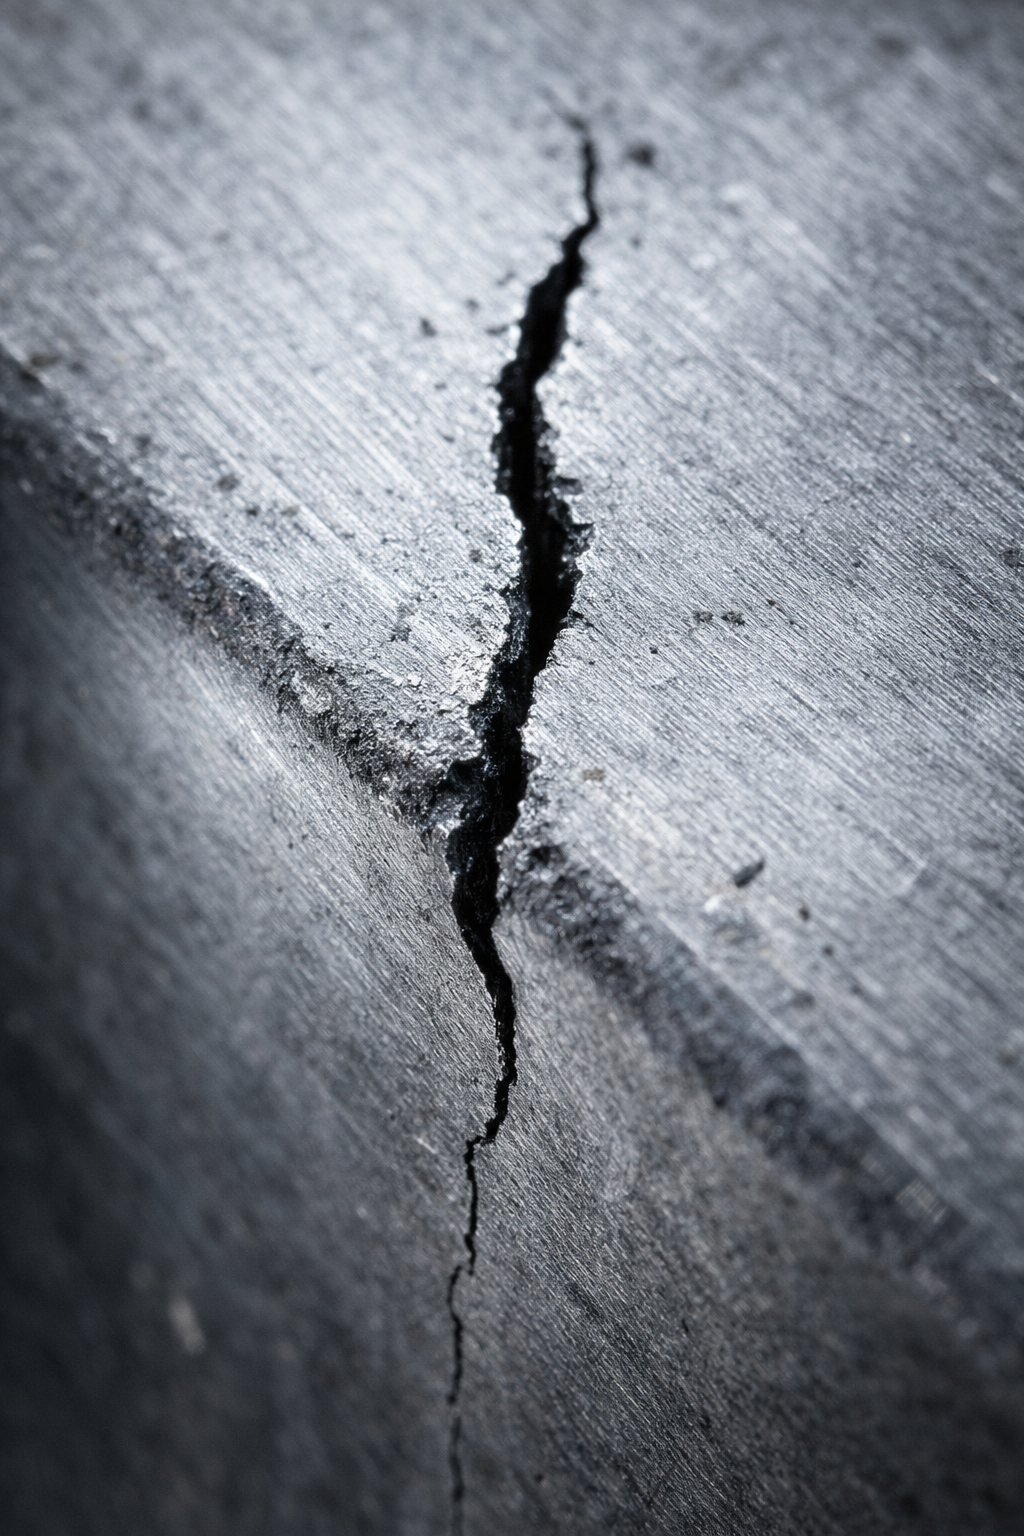
\includegraphics[width=0.62\linewidth]{bilder/haarriss.png}
	\caption{Hairline crack in a loaded metal surface. In many cases, such a crack does not arise suddenly, but through slow material fatigue. Over long periods, microscopic damage grows until a visible crack finally appears. This shows that mathematical models can capture the structure of the problem, while the concrete timing and path in reality often remain difficult to predict.}
	\label{fig:metallriss-haarriss}
\end{figure}

\newpage
\noindent

% =====================================================
% 10.9 Conclusion: Nature as Mathematical Structure
% =====================================================

\subsection{Conclusion: Nature as Mathematical Structure}

The examples in this chapter have shown
that mathematics in nature occurs not only in abstract formulas
or idealized figures.
It appears in real forms,
growth processes,
and orders:
in the honeycombs of the beehive,
in the branching of a tree,
in spirals of plants,
in the minimal surfaces of soap films,
in the symmetry of snowflakes,
and in the self-organization of dune landscapes.
Everywhere it becomes clear
that the visible world is not merely diverse,
but in many cases also mathematically structured.

Mathematical structure does not mean
that nature is built like a rigid textbook.
Real systems remain imperfect,
disturbed,
and shaped by many influences.
Precisely for this reason, the strength of mathematics lies not in exactly duplicating reality,
but in the ability
to make the supporting ordering principles visible
under changing conditions.
It does not show every detail,
but it makes understandable
why certain forms occur preferentially,
why growth follows certain patterns,
and why under given conditions certain structures
prove to be stable,
efficient,
or energetically favorable.

Thus the basic idea of this book gains new concreteness.
Mathematics is not only a tool of human thought
that is later applied to the world.
Rather, it is the means
by which we recognize the order
that is effective in the world itself.
Nature is not mathematically decorated,
but mathematically structured.

Precisely therein lies the deeper meaning of the examples considered here.
They show
that mathematical forms appear not only in theory,
but in reality --
not always perfectly,
not always ideally,
but clearly enough
for their structure to become recognizable.
From number through geometry to dynamics,
the same thought is confirmed again and again:
the world is not merely present;
it is ordered.
And mathematics is the language and form of knowledge of this order.

\medskip

This closes the arc of this book.
At the beginning stood numbers,
forms,
and the question
of whether mathematics is invented or discovered.
Through equations,
laws of nature,
abstraction,
chance,
complex dynamics,
philosophical interpretation,
and modern tools,
the path repeatedly led to the same insight:

Mathematics is not merely an aid
that human beings subsequently impose on the world.
It makes structures visible
that are effective in reality itself.

Nature is not perfect,
not ideal,
and not completely calculable.
But neither is it arbitrary.
In its forms,
processes,
symmetries,
limits,
and patterns,
an order becomes visible
that can be grasped mathematically.

This is precisely the central thought of this book:

\medskip

\begin{center}
	\emph{The structure of the world is mathematics.}
\end{center}